% Macros
\newcommand{\documenttype}{MÉMOIRE DE FIN D’ÉTUDES}
\newcommand{\submissiondate}{Lundi 2 Août 2021} 
\newcommand{\location}{Chatou} 
% //TODO : Modifier le titre du mémoire pour mieux coller au sujet
\newcommand{\documenttitle}{Sécurisation d’une infrastructure Kubernetes \linebreak et de ses applications}
\newcommand{\documenttitleun}{Sécurisation d’une infrastructure Kubernetes et de ses applications}
\newcommand{\documentauthor}{Lucas GRELAUD}
\newcommand{\corpmanager}{Marc BOUGET}
\newcommand{\documentreviewer}{David CHAMAILLARD}
\newcommand{\jurypresident}{ xxxxx XXXXX}

% config
%!TEX root = ./main.tex

\documentclass[
  paper=A4,
  fontsize=11pt,
  parskip=half,
  listof=totoc,
  draft=false,
  headings=small,
  oneside,
  final,
  numbers=noenddot
]{scrbook}

% Margins
\usepackage[
  left=25mm,
  right=25mm,
  top=20mm,
  bottom=30mm
]{geometry}

% Reduction of the spaces between headings and text
\RedeclareSectionCommand[afterskip=.0001\baselineskip]{section}
\RedeclareSectionCommand[afterskip=.0001\baselineskip]{subsection}
\RedeclareSectionCommand[afterskip=.0001\baselineskip]{subsubsection}
\RedeclareSectionCommand[beforeskip=.0001\baselineskip]{paragraph}

% Use UTF-8 char encoding
\usepackage[utf8]{inputenc}

% Font selection
\usepackage{fontspec}

% French spelling and French standard texts
\usepackage[french]{babel} 

% 1/2-line spacing
\usepackage[onehalfspacing]{setspace}

% For the use of graphics
\usepackage{graphicx}
\usepackage{wrapfig}

% Add tikz
\usepackage{tikz}
\usetikzlibrary{
    calc,
    positioning
}

% Better tables
\usepackage{tabularx}

% Diagonally divided table cells
\usepackage{diagbox}

% Table cells across multiple rows or columns
\usepackage{multirow}

% Multiple column page 
\usepackage{multicol}

% Possibility for line breaks in tables
\usepackage{makecell}

% Tables in landscape format
\usepackage{rotating}

% more line spacing in tables
\renewcommand{\arraystretch}{1.15}

% For the commands \ toprule, \ midrule and \ bottomrule, e.g. in tables
\usepackage{booktabs}

% Allows the use of colors
\usepackage{xcolor}
\definecolor{bluejcd}{RGB}{0,56,101}

% Links in PDF
\usepackage{hyperref}
\hypersetup{
  colorlinks=false,
  pdfborder={0 0 0},
  pdftitle=\documenttitleun,
  pdfauthor=\documentauthor,
}

% Improved URL handling with \ url {http: // ...}
\usepackage{url}

% Lists without spaces \ begin {compactlist} ... \ end {compactlist}
\usepackage{paralist}

% Allowing custom emunerate
\usepackage{enumitem}

% Output of the current time for the draft versions
\usepackage{datetime}


% Configuration of the figure and table names
\usepackage[
  format=hang,
  font={footnotesize, sf},
  labelfont=bf,
  justification=raggedright,
  singlelinecheck=false
]{caption}

% Macro for references under figures and tables
\newcommand{\source}[1]{\vspace{-.5\topsep}\caption*{\textsf{\textbf{Quelle:}} \textsf{#1}} }

% Place images at the exact location
\usepackage{float}

% Footnotes to headings
%\usepackage[bottom]{footmisc}

% Justification for caption
\usepackage[justification=centering]{caption}

% Quotes and bibliography
\usepackage[
    style=authortitle-ibid,
    giveninits=false,
    natbib=true,
    urldate=long,
    url=true,
    date=long,
    dashed=false,
    maxcitenames=2,
    maxbibnames=99,
    backend=biber,
    autocite=footnote,
    uniquelist=false,
    ibidpage=true,
    citetracker=true
]{biblatex}
\bibliography{library/library}
\DeclareLabeldate{
  \field{year}
  \field{date}
  \field{eventdate} 
  \field{origdate}
  \literal{nodate}
}
\AtEveryBibitem{
  \ifentrytype{book}{
    \clearfield{url}
    \clearfield{urldate}
    \clearfield{urlyear}
    \clearfield{urlmonth}
    \clearfield{urlday}
  }{}
  \ifentrytype{article}{
    \clearfield{url}
    \clearfield{urldate}
    \clearfield{urlyear}
    \clearfield{urlmonth}
    \clearfield{urlday}
  }{}
  \ifentrytype{inproceedings}{
    \clearfield{url}
    \clearfield{urldate}
    \clearfield{urlyear}
    \clearfield{urlmonth}
    \clearfield{urlday}
  }{}
  \ifentrytype{incollection}{
    \clearfield{url}
    \clearfield{urldate}
    \clearfield{urlyear}
    \clearfield{urlmonth}
    \clearfield{urlday}
  }{}
}


% Numbering level depth
\setcounter{secnumdepth}{3}

% Gliederungstiefe im Inhaltsverzeichnis 
\setcounter{tocdepth}{2}

% Level of detail in the table of contents
\setuptoc{toc}{totoc}

% List of tables and figures with designation
\usepackage[titles]{tocloft}

% Abbreviations
\usepackage{acronym}

% Suppress certain warnings
% see http://tex.stackexchange.com/questions/51867/koma-warning-about-toc
\usepackage{scrhack}

% Source code listings
\usepackage[chapter,newfloat]{minted}

\setminted{
  linenos=true,
  frame=lines,
  baselinestretch=1,
  breaklines=true,
  breakautoindent=true,
  fontsize=\small
}

\newenvironment{code}{\captionsetup{type=listing}}{}
\SetupFloatingEnvironment{listing}{name=Listing,listname=List of listing}

% Number footnotes consecutively
\usepackage{chngcntr}
\counterwithout{footnote}{chapter}

% UTF8 characters for math environment
\usepackage{amsmath}

% Improves the referencing of chapters, figures etc.
\usepackage[french,capitalise]{cleveref}

% Pandoc Integration
\providecommand{\tightlist}{%
  \setlength{\itemsep}{0pt}\setlength{\parskip}{0pt}}

% Define main font
\setmainfont{Arial}

% Define heading format
\tikzset{
  % Styling of header text is done using key/value options for TikZ nodes. See
  % section 16.4 of the PGF manual for a complete list of options that affect
  % text.
  headings/base/.style = {
    % Zap node seperation, set text width and alignment.
    outer sep = 0pt,
    % Trim off 2/3rd of an em to compensate for the inner xsep which spaces the
    % text nicely away from the left side, but causes the node to hang into the
    % right margin.
    text width = {\textwidth - 0.666em},
    align = left,
    text = white,
  },
  headings/chapter/.style = {
    headings/base,
    fill = bluejcd,
    font = \Large
  },
}

\newcommand{\colorboxedsec}[2]{%
  \tikz{\node[headings/#1]{#2};}}

\setkomafont{chapter}{\colorboxedsec{chapter}}

% Add figure caption with source
\newcommand*{\captionsource}[2]{%
  \caption[{#1}]{%
    #1%
    \\\hspace{\linewidth}%
    \textbf{Source:} #2%
  }%
}

% hyphenation
%!TEX root = ../main.tex

% declare hyphenation of words unknown to babel in this file like:
%  \hyphenation{hy-phe-na-tion}


\begin{document}
  %%%%%%%%%%%%%%%%%%%%%%%%%
  %% document title page %%
  %%%%%%%%%%%%%%%%%%%%%%%%%
  %!TEX root = ../main.tex


\begin{titlepage}

% Kensington picture
\begin{tikzpicture}[remember picture,overlay] 
    \node[anchor=north, yshift=-10mm] (jcd_pic) at (current page.north){
        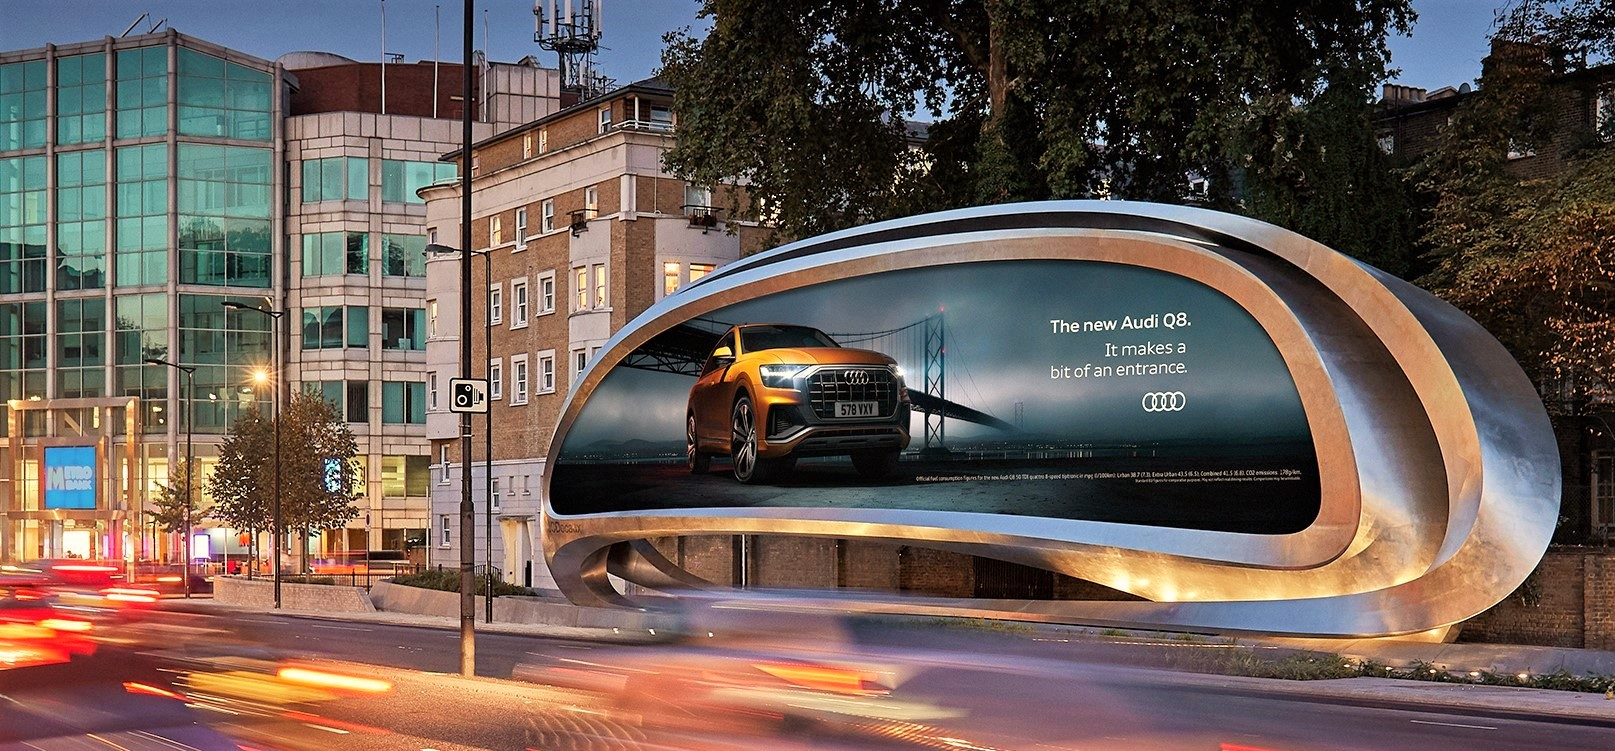
\includegraphics[width=0.9\paperwidth,height=0.45\paperheight]{resources/img/the_kensington_audi.jpg}
    };
\end{tikzpicture}

% Blue box (ugly way make it, but will do the job)
\begin{tikzpicture}[remember picture,overlay] 
    \node[anchor=north, yshift=-0.44\paperheight] at (current page.north){
        
\includegraphics[width=0.9\paperwidth,height=0.145\paperheight]{resources/img/blue_bg.jpg}

    };
    \node[anchor=north, yshift=-0.46\paperheight, xshift=-0.44\paperwidth, align=flush right, text width=0.7\paperwidth] 
    at (current page.north east) {
        \color{white} \Huge \textbf\documenttype\\
        \vspace{5mm}
        \color{white} \LARGE \documenttitle\\
    };
    \node[anchor=north, yshift=-0.64\paperheight, align=center, text width=0.7\paperwidth] at (current page.north) {
        \Large \textbf{Auteur:} Lucas GRELAUD\\
        \vspace{2mm}
        \Large \textbf{Période de mission :} 8 Février 2021 au 26 Août 2021
    };
    \node[anchor=north, yshift=-0.74\paperheight] at (current page.north) {
        \large
        \begin{tabular}{c@{\hskip 20mm}c@{\hskip 20mm}c}
    
            \textbf{\underline{Maître d'apprentissage}} & \textbf{\underline{Président du Jury}} & \textbf{\underline{Tuteur pédagogique}}\\
            \\
            \corpmanager & \jurypresident & \documentreviewer
        \end{tabular}
    };

\end{tikzpicture}

% ESIEA logo
\begin{tikzpicture}[remember picture,overlay] 
    \node[anchor=north, xshift=0.25\paperwidth] at (current page.north west){
        
\includegraphics[width=0.45\paperwidth,keepaspectratio]{resources/img/Logo_ESIEA_Baseline_blanc.png}
    };
\end{tikzpicture}

% Additionnal info
\begin{tikzpicture}[remember picture,overlay] 
    \node[anchor=south, yshift=-0.46\paperheight, xshift=-0.44\paperwidth, align=flush right, text width=0.7\paperwidth] 
    at (current page.south east) {
        \textbf\documenttype\\
        \vspace{5mm}
        \color{white} \LARGE \documenttitle\\
    };

\end{tikzpicture}

% JCDecaux logo
\begin{tikzpicture}[remember picture,overlay] 
    \node[anchor=south, yshift=15mm] at (current page.south){
        
\includegraphics[width=0.25\paperwidth,keepaspectratio]{resources/img/Logo_JCDecaux_seul_without_baseline.jpg}
    };
\end{tikzpicture}

\end{titlepage}



  %%%%%%%%%%%%%
  %% indexes %%
  %%%%%%%%%%%%%

  % disclosure statement - uncomment if needed
  % %!TEX root = ../main.tex

\addchap{Blocking notice}

This thesis may not be made accessible to third parties, with the exception of the supervising lecturers and authorized members of the administration, without the express consent of the company and the author.
In justified cases of suspicion, the thesis or parts thereof may be subjected by the FHDW to a plagiarism check by a plagiarism software provider and temporarily stored on FHDW-specific databases set up there.
The blocking notice is not effective in the event of a plagiarism check.
Reproduction and publication of the thesis without express permission - even in excerpts - is not permitted.

  % \newpage

  % executive summary - uncomment if needed
  %!TEX root = ../main.tex
\chapter*{Executive Summary}
It is farley known that the subject of computer security is a known issue the development of application by industries.
This issue is manly due to the fact that most of the development are side product of industries used to fulfil a 
technical need.
\newline This problematic is all the more significant when industries try to optimize their information system 
infrastructure by using containerized technologies and Cloud Computing at the same time.

In this thesis, we will try to find solutions and means to solve this ever-growing issue of securing the development and
deployment pipeline o containerized application. Then, after a careful selection, we will implement some of these solutions
on different parts of the pipeline and evaluate them.
\newline This work will also demonstrate the need of cooperation between security, architecture, infrastructure and 
development teams to achieve this goal.

The conclusion will follow with a first return of experience  of the implemented solution and associated results.
This par will include booth parts of  problematic.

Finally, we will discuss the future of the project and the possible tasks the company may need to accomplish to fulfil
its goal, more specifically on the training aspect.
  \newpage
  %!TEX root = ../main.tex
\chapter*{Résumé Analytique}
aaaaaaaaaaaaaaaaaaaaaaaaaaaaaaaaa
  \newpage

  % acknowledgment -  uncomment if needed
  % //TODO: Retirer // pour activer les remerciements
  %% //TODO : Remplir la page de remerciement

\chapter*{Remerciements}
Ce mémoire de mission de fin d'études constitue l'épilogue de trois riches et chaleureuses années d'apprentissage au sein de l'équipe de
sécurité du Groupe JCDecaux. C'est donc pourquoi je souhaiterais remercier 
  %\newpage

  % table of contents
  \tableofcontents
  \newpage

  %%%%%%%%%%%%%
  %% content %%
  %%%%%%%%%%%%%
  
  % insert chapter files here like this:
  %!TEX root = ../main.tex
\chapter{Introduction}

Cette mission de fin d'étude clôture trois années d'apprentissage réalisées au sein de l'équipe de sécurité informatique 
du Groupe JCDecaux. Elle permet aussi de finaliser un travail de longue haleine visant à sécuriser et moderniser
la chaîne de production des applications et outils exploités par le groupe et ses filiales.

\section{Le Groupe JCDecaux}
JCDecaux est un groupe industriel international fondée en France en 1964 par Jean-Claude Decaux et spécialisé dans 
l'affichage publicitaire urbain. Principalement connue pour son mobilier urbain (Abribus, MUPI\footnote{Mobilier Urbain 
Pour l'Information - Panneau d'affichage de 2m² dont l'une des faces est réservée pour les collectivités.}, Senior\footnote{
Panneau d'affichage de 4m² en fixation murale ou aérienne.}), l'entreprise familiale a su se hisser en tant que leader de 
la communication extérieure et est reconnue comme étant N°1 mondiale dans ce domaine depuis 2001. Le Chiffre d'Affaires du 
groupe était de 3 890.2 M€ en 2019.

La notoriété du Groupe JCDecaux s'explique par sa présence dans plus de 80 pays répartis sur tous les continents, mais
aussi et surtout par la qualité des services proposés tant auprès des collectivités locales qu'aux annonceurs.
Cette recherche de qualité, d'esthétique et d'innovation dans le mobiliers urbains fait partie intégrante des valeurs de 
l'entreprise et représente une réelle fierté pour ses 12 300 collaborateurs. 

\section{L'équipe Sécurité des Systèmes d'Informations}
\begin{wrapfigure}{R}{0.27\textwidth} 
    \centering 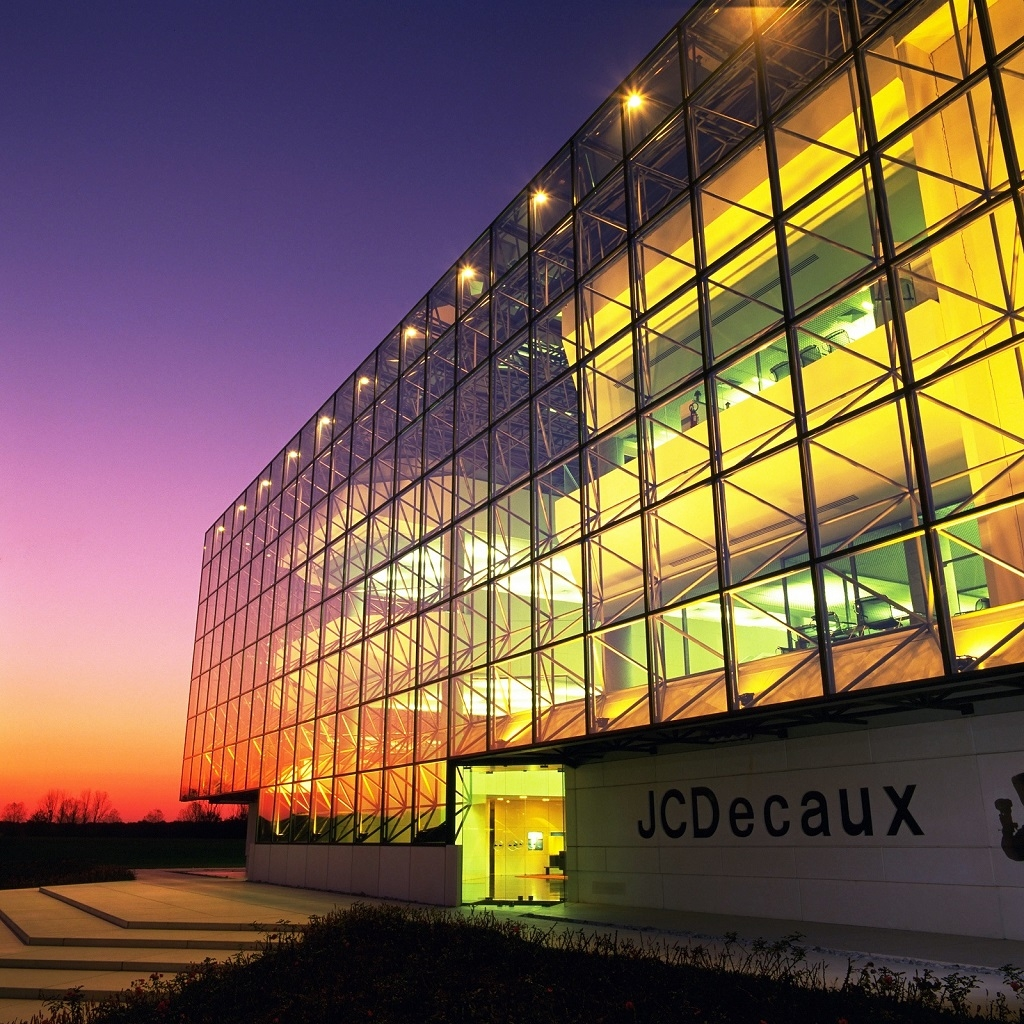
\includegraphics[width=0.25\textwidth]{resources/img/jcd_pla_front.jpg}
    \centering Siège de Sainte Apolline
\end{wrapfigure}
En 2013, la \ac{DSI} Groupe s'est pourvu d'une équipe dédiée à la \ac{SSI}.
Cette décision faisait suite à l'augmentation progressive des déploiements de systèmes de diffusion publicitaires numériques et
de la montée en puissance de la diffusion programmatique.

L'équipe \ac{SSI} Groupe de JCDecaux est localisée sur le plateau de la \ac{DSI}, au siège de Sainte-Apolline, Plaisir.
Elle est actuellement composée de trois personnels internes (le \ac{RSSI}, un ingénieur \ac{SSI}, un apprenti) et est complémenté 
par trois personnels externes en prestation.
\newpage
Les missions de cette équipe portent tant sur l'aspect organisationnel (Analyse de risque, gestion des politiques, sensibilisation),
l' opérationnel (SOC, conformité, veille phishing) que sur la qualification technique des systèmes et infrastructures. L'équipe propose
ainsi ces services au Groupe et à ses Filiales afin de sécuriser leurs systèmes.

\section{Publicité et développement applicatif}
De par la complexité et la volatilité du secteur publicitaire (publicité programmatique, booking de campagne, diffusion numérique), 
le Groupe JCDecaux se doit de disposer d'applications adaptées aux différents métiers de la publicité. 
Pour la réalisation de ces applications, le Groupe dispose d'équipes de développement interne dans une majorité des \ac{BU} 
de ses DSI (Groupe \& Filiales).

Depuis 2016, ces équipes de développement  ont mis en place dans leur projet des méthodes agiles; afin 
d'accélérer leurs temps de développement ainsi qu'améliorer la fiabilité et flexibilité de leurs applications.
Ce changement de doctrine sur les méthodes de gestion de projet a permis une réduction de la complexité des applications produites
grâce notamment à leur modularisation et favorise leurs réemplois pour tout ou partie dans les filiales du Groupe JCDecaux.

\section{Automatisation et conteneurisation du Si}
Conséquence de l'augmentation du nombre de composant applicatif dans le SI, le nombre de serveurs et machines virtuelles exploités par 
la \ac{DSI} n'a cessé de croître durant les cinq dernières années.

Pour palier à la complexité de gestion induite par cette augmentation, la \ac{DSI} Groupe s'est pourvu en outils et méthodes pour 
automatiser les tâches les plus courantes tel que l'initialisation des serveurs, le patch management ou encore le déploiement des
applications. Cet outillage a commencé par le développement et la mise en production d'une \ac{CMP} reliée à notre \ac{CMDB}, réel atout 
pour les équipes opérationnelles, puis la mise en place de script Ansible\footnote{Ansible est une plate-forme \ac{FOSS} développée par
RedHat servant à la gestion de déploiement applicatif au travers d'une simple connexion \ac{SSH}}

Depuis 2018, la \ac{DSI} Groupe et la \ac{DSI} France coopèrent dans un programme de déploiement des applications métier sous la forme
de conteneurs sur une infrastructure Kubernetes managé sur \ac{AWS}, le Cloud Provider de JCDecaux. Il vise à la simplification
déploiement applicatif en fournissant une couche d'abstraction unique et standard pour l'ensemble des équipes de développement du Groupe.

Ce programme est en phase de généralisation au sein du Groupe JCDecaux, mais un certain nombre de points relatif à la sécurisation des
applications, conteneurs et cluster Kubernetes sont à résoudre avant de pouvoir mettre cette technologie à disposition des filiales.

\section{Problématiques de sécurité}
Comme pour toute infrastructure hébergée par ou pour le Groupe JCDecaux, cette plateforme Kubernetes se doit de respecter un ensemble de 
règles et de principes définies par les IT Security Policies\footnote{FR: Politiques de sécurité Informatique}. Ces documents, 
regroupés par domaines (Réseau, Identité, Vulnérabilité, Données, etc..), régissent en effet l'aspect "Sécurité informatique" de tout projet
réalisés par les équipes du Groupe et les guides dans leurs développements.

Afin d'attester du niveau de conformité et de sécurité de la nouvelle plateforme, l'équipe \ac{SSI} à fait exécuter en externe un audit 
technique de cette dernière. Réalisé en Juillet 2020 par XMCO, cet audit avait pour objectif d'étudier le niveau de sécurité courant de 
l'environnement \ac{EKS} de JCDecaux (découverte et tentative d'exploitation de Vulnérabilités); ainsi que de fournir un certain nombre 
de recommandations visant à assurer la sécurité de la plateforme suite à sa généralisation.

Cet audit a permis de mettre en évidence de nombreuses de faiblesses et / ou défaut de conception de la plateforme Kubernetes. 
Suite à la restitution et analyse du compte-d'audit, plusieurs chantiers ont ainsi émergés :
\begin{enumerate}
    \item Cloisonnement de l'infrastructure
    \begin{itemize}
        \item Ségmentation des clusters en fonction des \ac{BU}
        \item Durcissement des règles réseau
    \end{itemize}
    \item Contrôle des déploiements
        \begin{itemize}
        \item Intégration de protection contre objets dangereux
        \item Application des PodSecurityPolicy
        \item Ajout de règles OpenPolicyAgent aux contrôleurs d'admission
    \end{itemize}
    \item Contrôle d'accès et secrets
    \begin{itemize}
        \item Renforcement du composant kube2iam
        \item Sécurisation du bastion SSH et des serveurs de rebonds
        \item Gestion et rotation des secrets
    \end{itemize}
    \item Sensibilisation et validation
    \begin{itemize}
        \item Mise en place de guides pour les développement / déploiement
        \item Sensibilisation des équipes
        \item Standardisation des déploiements
        \item Validation des images et des applications
    \end{itemize}
\end{enumerate}

\pagebreak

\section{La mission et ces objectifs}

Comme énoncé précédemment, quatre chantiers de remédiation sont à réaliser afin de rendre la plateforme Kubernetes conforme aux politiques
de sécurité informatique du groupe.

Le chantier de cloisonnement de l'infrastructure Kubernetes ainsi que celui relatif au contrôle d'accès sont en cours de 
finalisation. Ils ont en effet été lancés directement à la suite de l'audit.
\linebreak Le chantier de contrôle des déploiements est partiellement réalisé et celui de la sensibilisation reste à démarrer. C'est donc 
de à ces deux derniers que nous allons nous intéresser.

Les objectifs de ma mission de fin d'études sont exprimés de la façon suivante :
\begin{enumerate}
    \item Objectifs organisationnels : 
    \begin{itemize}
        \item Revue des procédures de qualification sécurité des applications, conteneurs et de déploiements
        \item Revue des procédures de gestion opérationnel de la sécurité des clusters Kubernetes
        \item Production de ressources visant à la standardisation des déploiements sur les clusters
        \item Production de guides et ressources visant à la sécurisation des développements pour Kubernetes
    \end{itemize}
    \item Objectifs techniques:
    \begin{itemize}
        \item Analyse des moyens techniques existants au sein du groupe et évaluation de leur efficacité.
        \item Consolidation et optimisation des moyens techniques existants.
        \item Qualification de nouvelles solutions techniques visant l’amélioration de la sécurité de l’infrastructure Kubernetes du  groupe, 
        tant sur les phases développements que sur les phases de déploiement.
        \item Intégration des solutions retenues à l’infrastructure. 
    \end{itemize}
\end{enumerate}

Ma mission est donc en réalité constituée de deux phases, chacune mêlant des objectifs organisationnel et techniques:
\begin{itemize}
    \item Première phase : revoir et normaliser notre méthodologie de gestion de la sécurité des développements (applicatif et conteneur)
    \item Second temps : fournir des éléments techniques et opérationnels visant à maintenir un bon niveau de sécurité dans l'exploitation 
    de la plateforme Kubernetes. 
\end{itemize}


  \newpage
  %!TEX root = ../main.tex
\chapter{État de l'art}
Deux sujets principaux seront abordés dans ce mémoire : la sécurisation d'une chaîne de production DevOps et la 
gestion opérationnelle de la sécurité d'une infrastructure \ac{K8S}.

Il me semble donc pertinent de présenter les risques de sécurité associés à ces deux sujets indépendamment afin de 
pouvoir mieux les définir et éventuellement démonter un certain recoupement avec d'autres problématiques de sécurité 
informatique. 


\section{Évaluation des risques de sécurité}

\subsection{Les risques du Pipeline DevOps}
Dans la méthodologie DevOps, le \emph{Pipeline} est un concept hybride regroupant des notions théoriques et un socle 
technique utilisés dans le cadre d'un développement logiciel. Ainsi, l'utilisation du terme \emph{Pipeline} fait aussi 
bien référence au \ac{SDLC} \autocite[Ch.\ 6]{devops_for_dummies_freeman_forsgren_2019}, aux standards de développement
\autocite[Ch.\ 9]{devops_for_dummies_freeman_forsgren_2019} , qu'au processus de qualification et validation, ou bien même
à l'ensemble des outils et services utilisés par les équipes de développement. 
\newline Il s'agit donc d'un élément central dans la chaîne de production DevOps: tout problème impactant un élément du 
\emph{Pipeline} aura des répercussions sur les autres et risque ainsi de mettre en péril les opérations de développement.

Nous pouvons donc nous poser la question de la nature des risques portés par le \emph{Pipeline}; et tout particulièrement
ceux portant sur l'aspect sécurisation informatique.
\newline Pour cela, nous allons utiliser comme support un \ac{SDLC} DevOps afin de mieux cibler les 
problématiques de sécurité à chaque étape d'un projet.

\vspace{0.5em}
\begin{figure}[h]
    \centering
    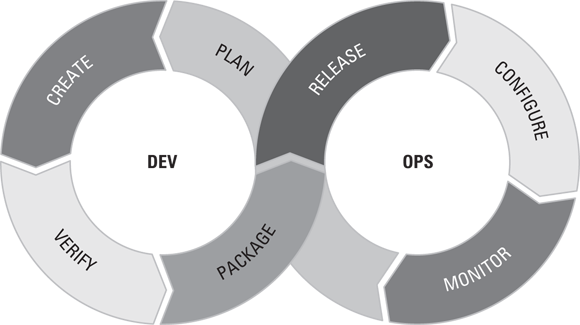
\includegraphics[width=0.5\linewidth]{resources/img/devops_lifecycle.png}
    \captionsource{Représentation du cycle de vie d'un projet DevOps}{DevOps for Dummies, Figure 6-1}
    \label{fig:devops-lifecycle}
\end{figure}
\newpage

Après une rapide analyse, voici les principaux risque qui se présente à nous :
\begin{multicols}{2}
    \begin{enumerate}
        \item Planification :
        \begin{itemize}
            \item Intégration d'une technologie vulnérable ou non maintenue
            \item Non-intégration de correctifs pour une vulnérabilité remontée
        \end{itemize}
        \item Conception :
        \begin{itemize}
            \item Développement de code faillible
            \item Mauvaise configuration du framework ou dépendances
        \end{itemize}
        \item Validation :
        \begin{itemize}
            \item Jeux de test incomplets
            \item Absence d'audit de sécurité applicative
        \end{itemize}
        \item Conditionnement :
        \begin{itemize}
            \item Utilisation d'un OS ou paquets vulnérables
            \columnbreak
            \item Erreur de configuration du conteneur
            \item Erreur de configuration des services
        \end{itemize}
        \item Livraison :
        \begin{itemize}
            \item Mauvaise gestion des versions de conteneurs
            \item Erreur de configuration du script de build
        \end{itemize}
        \item Configuration :
        \begin{itemize}
            \item Mauvaise gestion des secrets
            \item Erreur de configuration des déploiements
        \end{itemize}
        \item Surveillance :
        \begin{itemize}
            \item Absence ou trop faible collecte de traces (application et conteneur)
        \end{itemize}
    \end{enumerate}
\end{multicols}

On constate donc qu'une majorité des risques portés par le \emph{Pipeline} DevOps sont liés à des erreurs commises lors
du développement. Il s'agira donc d'un point d'attention dans la recherche de solutions.

\subsection{Les risques d'un cluster Kubernetes}
De par sa nature, l'orchestrateur \ac{K8S} et les nœuds qui constituent le cluster agissent comme une couche 
d'abstraction entre l'infrastructure du Cloud Provider et les conteneurs (aussi appelés \emph{Pods}) qu'il héberge.
\newline Il est cependant important de noter que quelques problématique de sécurité (\eg Réseau, accès API, chiffrement 
du traffic \emph{etcd}, \dots) sont tout de même à adresser. C'est en tout cas ce que recommande la documentation 
officiel de \ac{K8S}\autocite{k8s_security_2021}.

Nous nous retrouvons donc avec les risques propres au cluster \ac{K8S} qui, dans un certain sens, partagent des similitudes
avec les risques portés par des infrastructure virtualisés classique : Gestion du \ac{RBAC} et de l'authentification, 
gestion des secrets, qualité de service, etc..

Cependant, le fonctionnement d'un conteneur est différent d'une machine virtuelle : le kernel est partagé entre l'hôte et
le conteneur. De nouveaux risques apparaissent d'isolation d'environnements d'exécution et d'accès à des ressources 
sensibles apparaissent. 

\newpage

\section{Recherche de solutions}

Ayant identifié les risques encourus par notre Pipeline DevOps et l'infrastructure Kubernetes associée,
nous pouvons maintenant nous intéresser aux solutions permettant leurs réductions.

Pour cela nous allons utiliser comme support la méthodologie décrite dans le \citetitle{samm_v2.0_owasp_project_2021}
\autocite{samm_v2.0_owasp_project_2021}
de l'\citeauthor{samm_v2.0_owasp_project_2021}. Cette méthodologie, mise à jours, fait office de référence pour l'analyse
et l'amélioration de la sécurité des logiciels développés en entreprise.
\newline Elle est particulièrement recommandée dans le cadre de développement Agiles et / ou \linebreak DevOps.

\subsection{Le modèle de référence}

Le \ac{SAMM} est, comme son nom l'indique, un modèle permettant de quantifier le niveau de maturité d'un processus de 
développement logiciel sur le plan de la sécurité informatique. 

Cette quantification est réalisée sur la base de différentes pratiques de sécurité chacune regroupés dans des fonctions 
métier et notés sur une échelle de trois points avec en point initial zéro implicite. 
\newline Ces pratiques de sécurité disposent elles-mêmes de deux activités permettant de qualifier le niveau de maturité 
d'une entreprise sur les principaux thèmes associés à la pratique.

Le \ac{SAMM} peut donc être représenté de la manière suivante :

\begin{figure}[h]
    \centering
    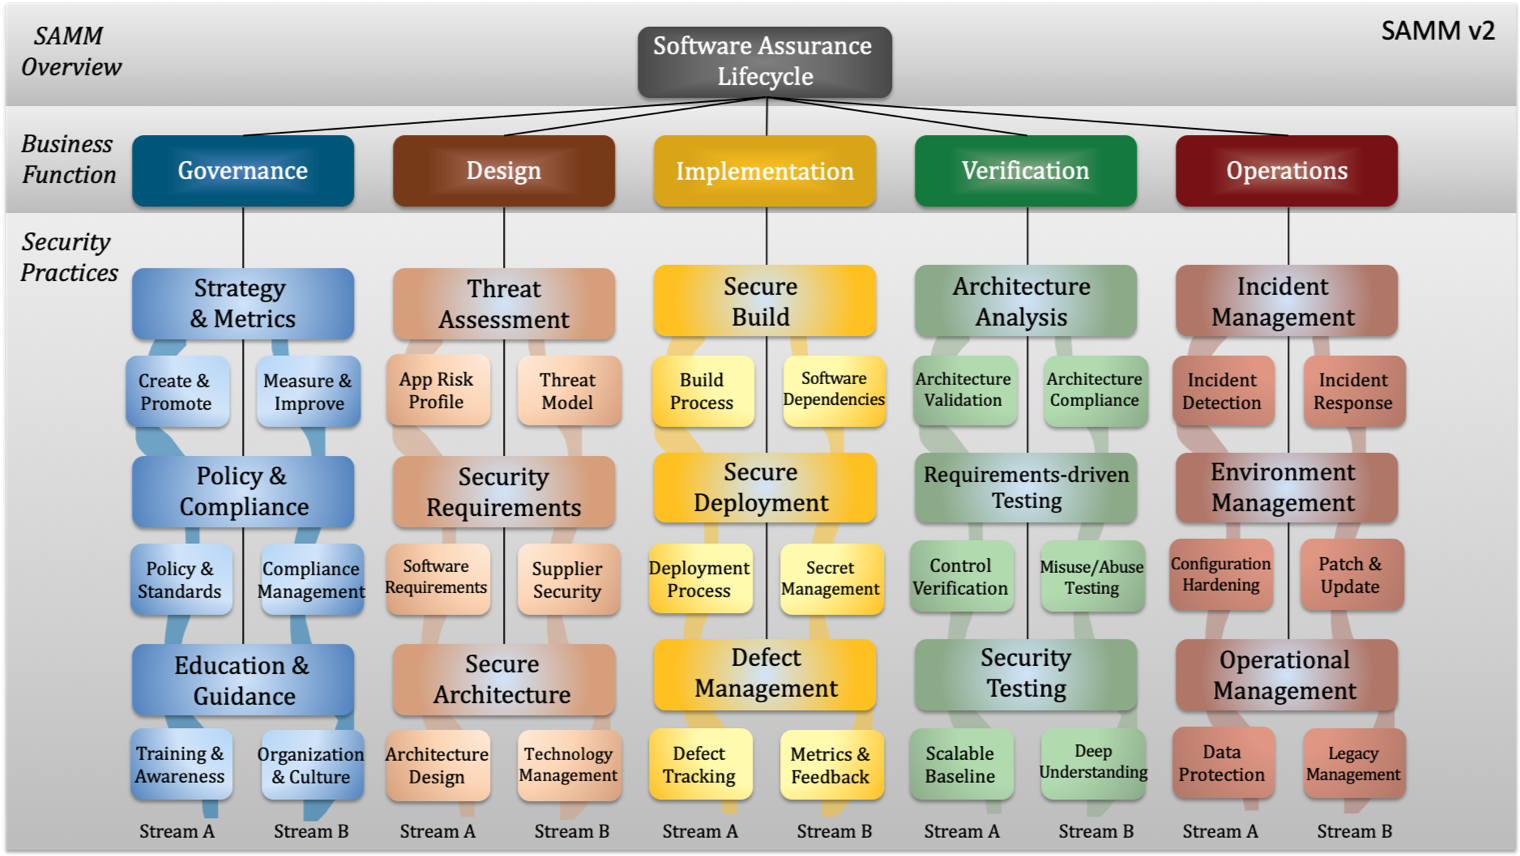
\includegraphics[width=1\linewidth]{resources/img/Samm_v2.png}
    \captionsource{Modèle SAMM v2}{Release note v2, \href{https://owaspsamm.org/release-notes-v2/}{OWASPSAMM.org}}
    \label{fig:samm-rep}
\end{figure}

\newpage

L'échelle de quantification quant à elle est définie de la manière suivante : 
\setlist[enumerate,1]{start=0}
\begin{enumerate}
    \item Niveau initial, aucune mesure de sécurité n'est appliqué.
    \item Niveau de compréhension basique de problématiques de sécurité et application de mesure ad hoc.
    \item Niveau avancé d'application des mesures de prévention avec constatation de l'efficacité ces dernières.
    \item Niveau de maîtrise complète des pratiques de sécurité à l'échelle de l'organisation.
\end{enumerate}
\setlist[enumerate,1]{start=1}
On considérera dans cette mission que le second niveau est un prérequis à la validation des pratiques de sécurité.
Le dernier niveau constitue quant à lui l'objectif à atteindre.

\subsection{Gouvernance}

La fonction \emph{Gouvernance}, telle que présentée dans le modèle \ac{SAMM}, représente le point de départ de la 
mise en œuvre de la sécurité informatique dans le cadre de développement. C'est en effet sur la base des 
trois pratiques de sécurité associés (\emph{Stratégie \& Métriques}, \emph{Politiquer \& Conformité}, 
\emph{Formation \& Conseils}) que seront issues l'ensemble des actions techniques et organisationnelles des autres
fonctions métier.

La \emph{Gouvernance} de la sécurité des développements est un sujet déjà encré dans la philosophie du Groupe JCDecaux.
Il dispose déjà d'un niveau de maturité avancé grâce à la mise en place de politiques de sécurité dédiées au 
applications et leur développement; à la formation et intégration d'interlocuteurs sensibilisés aux risques de sécurité;
de même que la mise en place de \ac{KPI} permettant la mesure et l'amélioration de l'efficacité de la stratégie.
\newline Cette stratégie, adoptant les principes de la sécurité par la conception (Security By Design) a par ailleurs 
fait  l'objet d'une présentation\autocite{devopsrex_denis_2019} lors du \href{https://2019.devopsrex.fr/}{DevOpsREX 219} 
par Joy-Alexandra Denis, ex-RSSI Adjointe du Groupe JCDecaux et maintenant RSSI Ikea France.

Cependant, et contrairement aux préconisations du \ac{NIST}\autocite*{app_cont_sec_nist_2017}, le Groupe ne dispose pas
d'une politique de sécurité dédiée aux technologies de conteneurisation d'application et d'hébergement connexe. 

De même, bien que l'on observe une forte sensibilisation aux problématiques de sécurité des responsables produit / 
projet, on constate que les populations de développeurs ne disposent pas d'un accompagnement spécifique et
institutionnalise au niveau du groupe sur ces \linebreak problématiques.

Ainsi, le \ac{SAFECODE} recommande la mise en place d'une formation continue des équipes de développement aux techniques
de sécurisation de code et au développement sécurisé dans son rapport \citetitle{six_pillarss_devsecops_safecode_2020} de 
\citedate{six_pillarss_devsecops_safecode_2020}.

\newpage

\subsection{Conception}

Si l'on considère que la \emph{Gouvernance} constitue les fondations d'un développement applicatif sécurisé, la 
conception et l'imagination de son architecture représente quant à elle l'ossature de cette dernière : une faiblesse dans 
la conception pourrait entraîner la compromission globale de l'application. 
\newline Afin de prévenir ces risques, le modèle \ac{SAMM} identifie trois axes de sécurisation : l'évaluation des risques, 
la définition de prérequis de sécurité et la sécurisation de l'architecture.

Depuis 2019, toutes les applications produites au sein du Groupe JCDecaux font l'objet d'une analyse de risques 
(voir annexe \ref{appendix:securitybydesign}) par les équipes de développement dès l'étude de faisabilité. 
Cette analyse de risques et les prérequis de sécurité associés seront ensuite soumis à une validation de l'équipe \ac{SSI} 
qui émettra des recommandations si cela est nécessaire.

Si certain prérequis de sécurité  dépendent directement de l'application développée, il est important 
de noter que la \ac{SAMM} et le \ac{SAFECODE}\autocite[p. 15]{fundamental_pract_sec_soft_safecode_2018} recommandent la 
mise à disposition des équipes de prérequis génériques pour les développement.
\newline Dans le cas du Groupe JCDecaux, ces recommandations sont présentées sous la forme de onze \emph{Golden Rules}
rédigés en anglais et disponibles pour toutes les équipes de développement du Groupe.

Enfin, il est conseillé de définir un set d'architectures applicative standards pour les développements. Cela peut prendre la 
forme d'une architecture Type ou d'une configuration modèle d'un framework .

\subsection{Implémentation}
L'implémentation, étape la plus chronophage dans un projet de développement, représente la principale activité des 
développeurs. C'est durant cette étape que ces derniers produisent le code source et ressources qui constitueront
l'application une fois compilée.

Afin de disposer d'une base commune de développement et de process, ces même développeurs mettent en œuvre divers outils
à unifier les environnements et d'automatiser le plus d'actions. On retrouve donc des outils de versionnage de code, 
d'exécution de tests automatiques ou bien encore de compilation et livraison automatique d'images\footnote{Ces outils de \ac{VCS}, 
\ac{CI}, \ac{CD} constituent dans les faits la base technique du Pipeline DevOps.}.

Ces outils étant performants et versatiles, la méthodologie \ac{SAMM} nous propose de les exploiter et ou complémenter 
afin de réaliser des opération d'évaluation de sécurité.
\newline Ainsi en intégrant des analyseurs de dépendances et en rajoutant des règles dans les profils d'évaluation de 
qualité de code, il est possible de drastiquement réduire le nombre de vulnérabilités d'un programme.
Dans le cas où l'intégration de ces règles serait trop coûteuse ou impossible, l'exploitation d'outils dédiés est 
envisageable. Ces outils sont des \ac{SAST}. 

Autre point important lors de l'implémentation, une gestion appropriée des configurations et des secrets est requise pour
toute conception d'application conteneurisée. En effet, il est primordiale de stocker ses configurations et secrets dans
un référentiel unique et auditable. Il en va de même pour les images conditionnées.

Cette centralisation des ressources par type permettra un meilleur suivi des défauts et par la suite la mise en place 
de \ac{KPI}. Ces \ac{KPI} pourront servir à l'évaluation des performances de sécurité des applications, mais aussi au 
ciblage des équipes nécessitant d'être accompagnées sur ce sujet.
\newline L'objectif final étant de pouvoir faire évoluer continuellement la gestion de la sécurité des applications grâce
à ces \ac{KPI}.

\subsection{Vérification}
Partie intégrante du développement applicatif, la phase de validation vise à tester toutes les fonctionnalités de 
l'application pour découvrir d'éventuellement dysfonctionnements.
\newline Dans le cadre de la méthodologie \ac{SAMM}, cette étape se présente sous la forme de trois pratiques de sécurité.

Dans un premier temps, il sera nécessaire de analyser l'architecture de l'application et de son implémentation dans le 
\ac{SI} à la recherche de vulnérabilités connues. Si aucun problème n'est détecté et que les mécanismes de sécurité de 
l'application sont corrects, nous pourrons passer à l'étape suivante.
\newline Dans le cas contraire, les développeurs devront appliquer des correctifs.

Dans un second temps, voir éventuellement en parallèle de l'étape précédente, il sera nécessaire de faire exécuter des 
test d'intégration continue afin de valider le bon comportement de l'application vis à vis de vulnérabilité connue.
Des test de charge et d'attaque sur la logique métier de l'application sont par ailleurs fortement recommandées.
\newline Des solutions de \ac{DAST}  et \ac{IAST} tel que les services \href{https://www.rapid7.com/products/insightappsec/}
{Rapid7 InsightAppSec} et \href{https://www.acunetix.com/}{Acunetix d'Invicti} peuvent donc se montrer fort intéressantes.

Enfin, si et seulement si aucun problème n'a été détecté, alors nous pourrons lancer un audit de sécurité (aussi appelé 
\emph{pentest} pour Penetration Testing). Cet audit devra être réalisé sur une instance d'application iso-production afin
de coller le plus possible à l'intégration finale. Un environnements de d'intégration ou de pré-production est donc le 
plus adapté.

Pour le Groupe JCDecaux, on constate une certaine déviation vis à vis des recommandations de la méthodologie \ac{SAMM}.
Si la validation de l'architecture et les audits de sécurité sont bien réalisés, la portion \ac{DAST} / {IAST} n'est 
quant à elle pas présente.

\subsection{Opérations}
Si jusqu'ici les différentes solutions proposées par la méthodologie \ac{SAMM} et le groupe \ac{SAFECODE} portaient sur
la sécurisation du \emph{Pipeline} DevOps, cette dernière fonction métier se concentrera essentiellement la sécurisation
de l'exploitation de l'application développée, et donc du cluster l'hébergeant.

Le premier aspect de sécurité opérationnelle à résoudre porte sur la façon dont un conteneur fonctionne sur le cluster.
Ainsi, il est nécessaire de pouvoir durcir les configurations d'exécutions des pods, soit en fournissant des outils de 
configuration automatique, soit en  appliquant des point de contrôle bloquant lors du déploiement d'un conteneur sur un 
cluster.

Deuxième aspect d'importance, la connaissance des pods en cours d'exécution sur un cluster ainsi que la connaissance de
leur état de vulnérabilité est primordial à la sécurisation du cluster. Ainsi, comme pour les infrastructures "classiques",
l'exploitation de scanner de vulnérabilité est une nécessité pour disposer d'informations suffisantes et fiables pour
avoir une gestion appropriée des patchs de sécurité.

De même que le besoin se fait sentir pour les infrastructures virtualisées, la gestion des incidents sur les clusters doit 
être efficace et proactive. Cela sous-entend d'avoir à disposition une procédure décrite de manière exhaustive et connue
par les équipes en lien avec la plateforme.

La première source d'information pour la gestion d'incidents sera les logs applicatifs et issues du cluster, 
bien que ceux-ci peuvent être complémentés par des informations liées au fonctionnement du conteneur. C'est par exemple 
ce que propose la solution \href{https://sysdig.com/opensource/falco/}{Falco (Sysdig)}.
\newline La création d'un inventaire exhaustif des pods en cours d'execution et de leur état de vulnérabilité
constituera quant à lui la deuxième source d'information pour la gestion opérationnelle de la sécurité des clusters 
\ac{K8S}.

Enfin, un travail proactif de gestion des systèmes dit \emph{legacy} et / ou en fin de vie devra être réalisé; pour les
mêmes raisons qu'il est réalisé sur l'infrastructure physique et virtualisés.

\newpage

\section{Analyse et critique des solutions}

Pour cette étude, nous nous sommes appuyés sur l'exploitation de deux principaux documents de référence : le rapport 
\citetitle{fundamental_pract_sec_soft_safecode_2018} (SAFECode) et la documentation officielle de la méthodologie 
\citetitle{samm_v2.0_owasp_project_2021} (\ac{OWASP}). 

Nous pouvons donc nous questionner sur la correspondance des solutions apportées par ces documents et les 
problématiques posées par notre mission.

\subsection{Les sources de l'étude}
Comme présenté ci-dessus, deux principales sources ont été utilisées lors de cette étude, les sources secondaires servant
à appuyer un point ou donner des éléments de réponse complémentaires.

Ce faible nombre s'explique par le fait que ces deux ressources font office de référence pour une majorité des études et 
guides d'implémentation de sécurité dans un processus de développement applicatif. On retrouve en effet référence à ces
documents dans les publications \citetitle{ssdf_nist_2012} (\ac{NIST}) et \citetitle{sage_carnegie_mellon_university_2021}
(Carnegie Mellon University Software Engineering Institute) qui m'ont servi de support d'implémentation dans mes missions.

C'est donc  pourquoi j'ai fait le choix de concentrer la recherche des solutions aux problématiques de ma mission autours
de ces deux seuls documents.

\subsection{Les solutions présentées}
Les solutions présentées dans cette étude de l'état de l'art de la sécurisation d'un processus de développement et 
déploiement applicatif sont agnostiques des technologies et techniques exploitées. Elles sont en effet formulées de façon à
pouvoir être mises en œuvre tant dans un contexte de développement classique que DevOps.
\newline De ce fait, il sera nécessaire d'intégrer et d'adapter ces solutions aux \emph{Pipelines} présents au sein 
du Groupe JCDecaux et de ses filiales.

De plus, cette étude nous présente un nombre conséquent de solutions, portant tant sur des sujets organisationnels que
techniques. Une sélection des solutions devra donc être réalisée afin que celles-ci correspondent au mieux aux problématiques
de la mission et que leur intégration puisse être réalisé dans le temps imparti à cette dernière.

Une attention particulière devra être portée sur les projets en cours de réalisation au sein de la \ac{DSI} Groupe afin de mieux 
coordonner les actions; notamment vis-à-vis des sujets liés à l'analyse de risques. 

\newpage


\subsection{Impact du COVID-19}
Comme pour beaucoup d'entreprises du secteur de la publicité, la crise du COVID-19 a eu un impact considérable sur le
marché. Cet impact s'exprime par une chute massive des commandes de diffusion de campagnes publicitaires et donc du 
chiffre d'affaire.
\newline Pour le Groupe JCDecaux, cette perte est estimée à -40,6\% du chiffre d'affaire pour l'année fiscale 2020; soit
une perte 2 311,8 millions d'euro\autocite{jcdecaux_resultfin_2020}.

Afin de réduire les effets de cette perte d'activité, des mesures de restriction des coûts et de sauvegarde d'emplois 
ont été mises en œuvre au sein du Groupe et de ses filiales. L'ensemble des équipes du Groupe et une majorité des équipes
de la filiale France se sont donc retrouvés en activité partielle (70\% temps travaillé et 30\% de chômage partielle) 
dès le mois de Mars 2020. Ces mesures sont encore effectives à lors de la rédaction de ce mémoire.

\section{Conclusion et solutions retenues}
Grâce à cette étude d'état de l'art portant sur la sécurité des développements et déploiements applicatif, nous pouvons 
constater que nombreuses sont les solutions aux problématiques posées par le sujet. 

En effet, ce sujet est à l'étude par des organismes de recherche, des administrations et organisations à but 
non lucratif depuis près de quinze ans. Nous disposons donc d'un certain recul sur le sujet et ce même si les 
problématiques de conteneurisation sont relativement nouvelles ( +/- 5 ans).
C'est par ailleurs pourquoi certaines de ces problématiques sont déjà adressées pour le Groupe.

Cependant, compte tenu du contexte dans lequel est réalisé ce mémoire, certaines solutions qui devraient être mises en 
œuvre nous pourront pas être intégralement implémentée à cause de leur coût ou par manque de ressources (humaines / 
temps).

C'est pourquoi nous allons nous concentrer sur la résolution des solutions suivantes : 
\begin{itemize}
    \item Création d'un processus de qualification sécurité des applications
    \item Création de politiques de sécurité dédiées aux conteneurs et à leur déploiements
    \item Mise à disposition d'outils d'évaluation de la sécurité de conteneurs
    \item Création d'un processus opérationnel de gestion de la sécurité des clusters
    \item Mise à disposition d'outils d'inventaire et de suivi de vulnérabilités pour les clusters
    \item Évaluation de la sécurité de la plateforme de gestion des configurations
    \item Durcissement des conteneurs et de leurs déploiements
\end{itemize}
  \newpage
  %%%%%%%%%%%%%
  %% closing %%
  %%%%%%%%%%%%%
  
  % acronyms
  %!TEX root = ../main.tex

\addchap{Liste des acronymes}

\begin{acronym}[ABCD]
	% declare your own acronyms here:
	\acro{RSSI}{Responsable de la Sécurité des Systèmes d'Information}
	\acro{SSI}{Sécurité des Systèmes d'Information}
	\acro{DSI}{Direction des Systèmes d'Information}
	\acro{SOC}{Security Operation Center}
	\acro{AWS}{Amazon Web Services}
	\acro{BU}{Business Unit}
	\acro{CMP}{Cloud management Platform}
	\acro{CMDB}{Configuration Management DataBase}
	\acro{K8S}{Kubernetes}
	\acro{SI}{Système d'Information}
	\acro{SDLC}{Software Development Life Cycle}
	\acro{SAMM}{Software Assurance Maturity Model}
	\acro{RBAC}{Role-Base Access Control}
	\acro{KPI}{Key Performance Indicator}
	\acro{NIST}{National Institute of Standards and Technology}
	\acro{SAFECODE}{Software Assurance Forum for Excellence in Code}
	\acro{IAM}{Identity and Access Management}
	\acro{VCS}{Version Control Sytem}
	\acro{CI}{Continuous Integration}
	\acro{CD}{Continuous Delivery}
	\acro{SAST}{Static Application Security Testing}
	\acro{DAST}{Dynamic Application Testing}
	\acro{IAST}{Interactive Application Security Testing}
	\acro{OWASP}{Open Web Application Security Project}
	\acro{BPMN}{Business Process Model and Notation}
	\acro{DAF}{Directeur Administratif et Financer}
	\acro{npr}{non-production}
	\acro{ECR}{Elastic Cloud Registry}
	\acro{ACL}{Access Control List}
\end{acronym}
  \newpage

  % list of figures
  %\listoffigures
  %\newpage

  % list of tables
  %\listoftables
  %\newpage

  % list of listings
  %\listoflistings
  %\newpage
  % list of references
  %!TEX root = ../main.tex

\addchap{Références}

\defbibheading{book}{\section*{Monographien}}
\defbibheading{article}{\section*{Beiträge in Zeitungen und Zeitschriften}}
\defbibheading{incollection}{\section*{Beiträge in Sammelbänden}}
\defbibfilter{incollection}{
    type=inproceedings or    
    type=incollection or
    type=inbook
}
\defbibheading{paper}{\section*{Papers}}
\defbibfilter{paper}{
    type=thesis or
    type=report
}
\defbibheading{online}{\section*{Internetquellen}}
\defbibheading{jurisdiction}{\section*{Rechtsprechung}}
\defbibheading{company}{\section*{Unternehmensunterlagen}}
\defbibheading{uncited}{\section*{Unzitierte Quellen}}
\defbibcheck{uncited}{
  \ifciteseen
    {\skipentry}
    {}
}

\setlength\bibitemsep{1.5\itemsep}
\setlength{\bibhang}{2em}

\begingroup
\sloppy

\printbibliography[heading=book,type=book]
\printbibliography[heading=article,type=article]
\printbibliography[heading=incollection,filter=incollection]
\printbibliography[heading=paper,filter=paper]
\printbibliography[heading=online,type=online]
\printbibliography[heading=jurisdiction,keyword=jurisdiction]
\printbibliography[heading=company,keyword=company]
%\printbibliography[heading=uncited,check=uncited]
%\nocite{*}

\endgroup

  \newpage

  % appendix - uncomment if needed
  %!TEX root = ../main.tex

\addchap{Appendix}
\label{appendix}

% create a table of appendices here manually like this:
%  \contentsline{section}{\numberline{1}AppendixTitle}{\pageref{app:appendixlabel}}{app:appendixlabel}

\newpage

% input the appendix files here like this:
%  \input{appendix/appendix1.tex}
%  \newpage

  \newpage

  % affirmation
  %%!TEX root = ../main.tex

\addchap{Declaration on honorg}

I hereby declare that I have prepared this thesis independently.
Only the sources and aids expressly named in the thesis have been used.
I have marked as such any ideas taken over verbatim or in spirit.
This work has not yet been submitted to any examination authority in the same or a similar form.
\vspace{20mm}

\location, \submissiondate
\vspace{10mm}

\underline{\hspace{8cm}}\\\documentauthor

\end{document}
